\documentclass{article}
\usepackage[utf8]{inputenc}

\usepackage{natbib}
\usepackage{graphicx}
\usepackage{wrapfig}
\usepackage{subcaption}
\usepackage{float}
\usepackage{hyperref}
\hypersetup{
    colorlinks=true,
    linkcolor=blue,
    filecolor=magenta,      
    urlcolor=cyan,
}

\begin{document}


\title{Deep Learning Autonomous Lab 1 \\
    \large Comparing optimization functions}

\author{Santiago Bernal }
\date{April 2018}


\maketitle
\newpage

\section{Introduction}
One of the largest concerns when designing a neural network is getting stuck in a “local minimum” when solving large scale non-convex optimization, where the  minimization of the model’s loss function reaches a small gradient, but it is still not at the lowest point reachable. Although more advanced neural networks and a deep architecture seem to avoid this problem, they still face challenges when reaching saddle points or plateaus \citep{GoodfellowV14}.

\begin{wrapfigure}{r}{0.4\textwidth}
 \vspace{-10pt}
  \begin{center}
    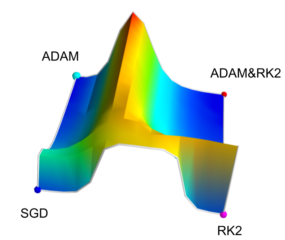
\includegraphics[width=0.3\textwidth]{NIN_3D_sgd_adam_RK2s-300x290.png}
  \end{center}
  \caption{NIN CIFAR10}
\label{fig:nincifar10}
\end{wrapfigure}

The main issue that has been detected is how the initial configuration can affect the results and how different algorithms can sometimes find different minimums, since they have different ways of dealing with saddle points, as is shown on figure \ref{fig:nincifar10} \citep{ImTB16}. The figure shows a  "visualization of the loss surface at weights interpolated between the final points of four different algorithms from the same initialization", using a Network-in-Network feed-forward convolutional networks for image classification of the CIFAR10 dataset \cite{Krizhevsky09learningmultiple} and projecting the outcomes on low dimensional sub-spaces based on initial and final weights configuration of the network. The final points are local minimums in the projected space, but it is not easily visualized if it is a local minimum as well in the high dimensional space, still, the difference between the different algorithms is easily observable.
\\
In this lab we will explore the optimization effects of different algorithms on test functions and simple datasets, and compare to how they work on deep neural networks using the Keras: "Reuters newswire topics classification" dataset.

\section{Comparing Optimizers}
\subsection{Optimizers with Test Functions}
Test functions, also known as artificial landscapes, are used to evaluate different characteristics of optimization algorithms by posing typical situations which they will have to face. 

\begin{figure}[H]
    \centering
    \begin{subfigure}[b]{0.7\textwidth}
        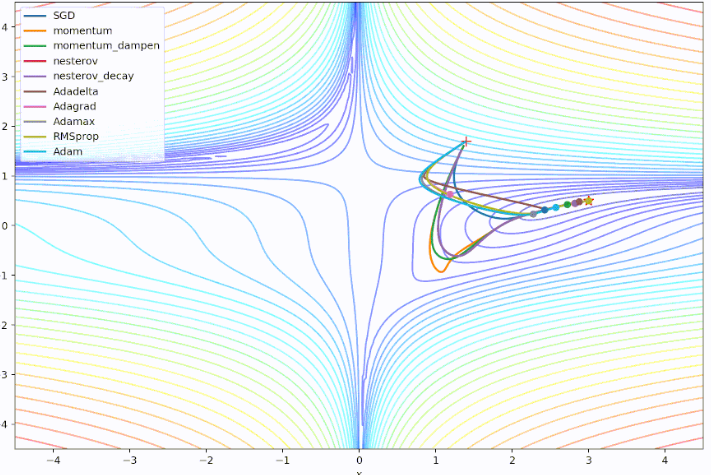
\includegraphics[width=\textwidth]{beale.png}
        \caption{Beale}
        \label{fig:beale}
    \end{subfigure}
     %add desired spacing between images, e. g. ~, \quad, \qquad, \hfill etc. 
      %(or a blank line to force the subfigure onto a new line)
    \begin{subfigure}[b]{0.7\textwidth}
        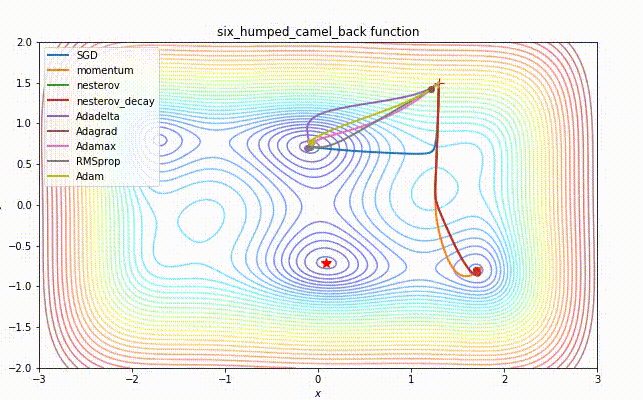
\includegraphics[width=\textwidth]{sixhumpedcamel.png}
        \caption{Six humped camel}
        \label{fig:sixhumpedcamel}
    \end{subfigure}
    \caption{Optimization on test functions \cite{clark_2017}}\label{fig:optimizationtestfunctions}
\end{figure}

The beale function is a multimodal function, characterized by having sharp peaks at the corners \cite{surjanovic_bingham_2017}. Using various optimizers on this function as seen on figure \ref{fig:beale}, shows how some algorithms find a direct path, others sway a bit before, and some take longer to reach the minimum, but overall they all find their way towards the minimum. Additionally, momentum based algorithms seem to head towards the minimum as if it was a ball heading down a slope. An animated view of the the optimization \cite{clark_2017} shows that the adaptive methods tend to reach the minimum faster.\\
On the other hand, using the six-hump camel function, which has six local minimums and two global \cite{surjanovic_bingham_2017_2}, it is more evident how different algorithms work around local minimum, with two of them (momentum, nesterov decay) getting stuck and not reaching the global minimum. It is also worth noting that the SGD method corrected its trajectory and ended up heading the right way.

\subsection{Comparing with moons}


\begin{figure}[H]
 \vspace{-10pt}
  \begin{center}
    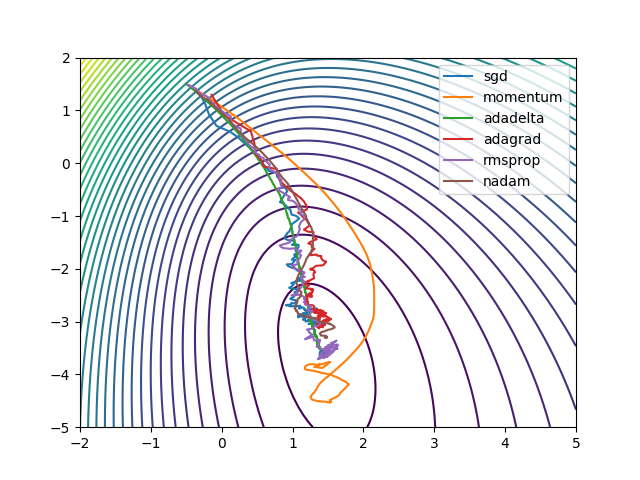
\includegraphics[width=0.9\textwidth]{moons1.png}
  \end{center}
  \caption{Optimizations on moon dataset}
\label{fig:moon}
\end{figure}


Using sklearns make moons dataset \cite{scikit-learn} which consists of two interleaving half circles, and using tensorflow \cite{tensorflow2015-whitepaper} for the different optimizers based on Alec Radford's animations \cite{yuret_2015}, we are able to view how they work on real datasets. For this, we use sigmoid cross entropy as a loss function, and use the optimizers to minimize the results, and then graph each iterations result over the loss contour. One of the main problems found in this case is how different parameters affect how each algorithm reaches the minimum, they had to be fine tuned in order for them to reach the final point in the best way possible. For example, the adadelta optimizer required a high amount of iterations (2500) for it to reach the minimum (using the recommended parameters: learning rate=1.0, rho=0.95 and epsilon=1e-6 \cite{adadelta}), lower values would mean that the minimum was never reached. The reason this may happen with adadelta is because of its slow start because of the accumulation of the square of the updates, considering that at the beginning this accumulative is 0. Even though this happens, after some amount of iterations (around 2000) it speeds up drastically. When changing the epsilon parameter, for a bigger amount (1e-3) the performance is similar to the adagrad method.

Similar to figure \ref{fig:beale} the momentum algorithm go around the final point and then fall on it as if it where a ball heading down a slope. In this case, the rest of the algorithms work in a similar way to each other after the fine tuning, each moving side to side and heading down the slope and reaching the global minimum, which shows the dynamics of the minibatches. The other exception is adadelta which heads in a more direct line towards the minimum when using the default parameters and 2500 iterations. This can be viewed in the figure \ref{fig:moon}.

\subsection{Comparing using deep neural networks}
\subsection{Using Reuters Newswire Dataset}
The Keras reuters newswire dataset, consists for 11.228 newswires from Reuters labeled over 46 topics. Each wire is encoded as a sequence of word index, where each word is indexed as the overall frequency of the word in the dataset, in a way that "3" is the third most frequent word, unknown words are encoded as "0". The dataset is of sequential type, which means that data items are stored consecutively, therefore it is of one dimension, where each member is a list of indexes. The dataset was splitted into 70\% train, 10\% validation and 20\% testing. To be able to use this dataset, we need to convert it from a sequence to a matrix since we are using a Feed-Foward Neural Network design. For this, the "Tokenizer" from Keras was used to vectorize it, a maximum of 5000 words where chosen to be processed, considering that a low amount or a large amount of words would make it too complicated for the model to be accurate or perform well. A low amount of words means that the model can't correctly establish why the classification is chosen for the different samples, given that there is no pattern or relationship that can be established between the word and the result. It tries to predict the newswire topics based on one word, which is really hard, this is evidenced in the figure \ref{fig:ovlowwords}. When a high amount of words is used, the model has more options on which to make predictions on which means that it may reduce accuracy for cases where there are not too many examples present for it to detect patterns. Also, the processing for a large amount ends up using a lot more computational time that is not needed, since some words are insignificant to the newswire topic (for example, words like "a", "the", "it", etc). For this dataset, having a high amount of words (30000) resulted in high accuracy (figure \ref{fig:rhmw}) but the model takes a lot of time to train \\
When obtaining the matrix from the sequence, the resulting size is [length of sequences, number of words] which in this case would be [8982, 5000] for the training data and [2246, 5000] for testing. The way the method vectorizes the sequence can be done by various modes: binary, which is if the word is present or not in the sample; count which is the amount of times a word is repeated; tfidf is the word frequency inverse document frequency, which reflects how important a word is to the sequence; and freq which is its frequency. Using the binary mode, we can establish a relationship with the word and the topics which will help classify the data based on the appearance of a word, which is what we want. Modes like count or frequency can lead to inaccurate results considering that articles like "a", "the" are going to be very common, and do not determine the classification, but in this case it may create invalid bias in the model. Finally, the class vectors returned by Keras are turned to a binary matrix in order to use it for calculating softmax, which is the output layer activation function.

\subsection{Creating the model}
After configuring the dataset, the model to be used needs to be defined. For the input layer, the input is the words found on the previous step (the binary result), so the input size is going to be the number of words to be processed defined previously. The final output layer, has the number of classes of the dataset as output and softmax as an activation function. The output of the input layer and the different hidden layers to use and their properties are more arbitrary to decide. A general rule of thumb used is that the amount of neurons for the hidden layers should be lower than the input and higher than the output, a value somewhere in the middle. This makes sense as well for this dataset, for example, considering that we want to establish relationships between the words and the topics, adding more neurons to a layer than the amount of neurons we have as input will make the network establish weird relationships between a word and a topic that doesn't exist so the network won't learn appropriately. As for the amount of hidden layers to use, usually one hidden layer can adapt to most feed-forward network architectures, sometimes two hidden layers can work out learning more detailed information.\\
Based on this, the model designed for this dataset would be of two hidden layers, one with 2048 neurons and another of 512 neurons, both using 'relu' as the activation function. Even though this dataset can still obtain good results with one hidden layer \ref{fig:rol}, two where chosen since the optimizations are going to be compared using a deep model. The amount of neurons for the first layer was chosen as the closest power of 2 in the average of the input (5000) and the output (46), which resulted in 2048, and then the same with the second hidden layer, resulting in 512.

\subsection{Training and results}
Having the dataset formatted and the model designed, the training could start, but first, a few other parameters had to be established: the batch size and the amount of epochs. For the batch size, its important to consider that a big batch can tend to converge to sharp minimizers which lead to poor generalization. Small batches, on the other hand, converge to flat minimizers which may be due to inherent noise in gradient estimations (mostly affects SGD) \cite{KeskarMNST16} and would take a lot more time to train the model. For this dataset, SGD is mostly affected by the batch size (figures \ref{fig:rsb} and \ref{fig:rlb}) where a large batch size got the optimization stuck in a local minimum without reaching the global minimum, this was avoided using smaller batch sizes. Usually, values like 32, 64 and 128 are chosen, for this case, 32 was used, which results in interesting characteristics in the optimization functions. As for the amount of epochs, this parameter is usually determined when a network reaches a minimum and no longer improves, but for this case, a low amount of epochs (5) where chosen to be able to point out different results of the optimizations easier. \\
Now that all the parameters where established, the model can be trained. We used the optimization methods: sgd, adam, adadelta, adagrad, adamax, nadam and rmsprop to minimize the loss function and the results shown on figure \ref{fig:rfm} where obtained.

\begin{figure}[H]
    \centering
    \begin{subfigure}[b]{0.7\textwidth}
        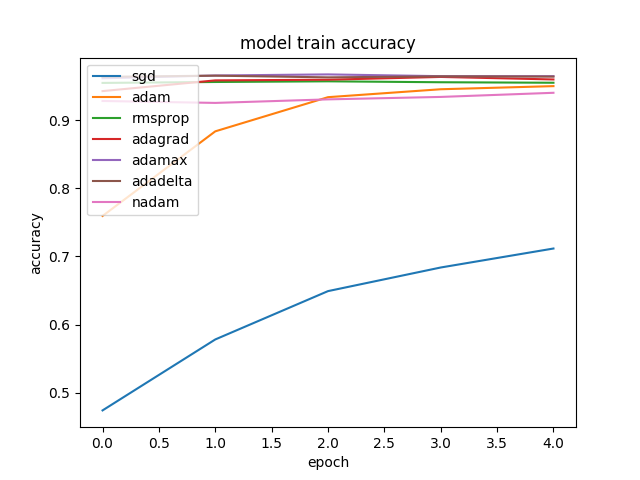
\includegraphics[width=\textwidth]{2layer20418-512-trainacc.png}
        \caption{Train accuracy}
        \label{fig:tafm}
    \end{subfigure}
     %add desired spacing between images, e. g. ~, \quad, \qquad, \hfill etc. 
      %(or a blank line to force the subfigure onto a new line)
    \begin{subfigure}[b]{0.7\textwidth}
        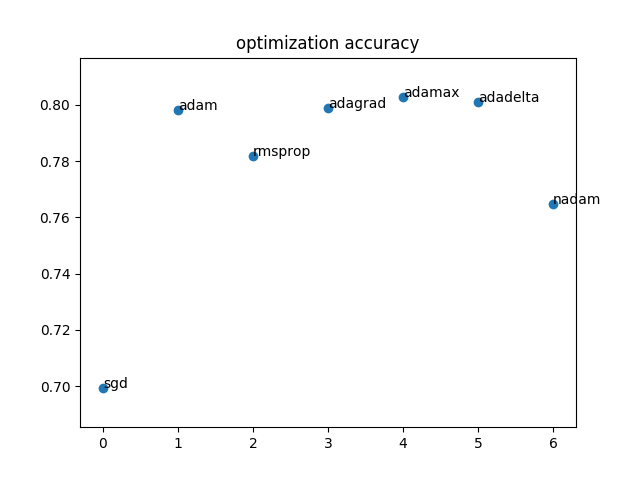
\includegraphics[width=\textwidth]{2layer2048-512-testacc.png}
        \caption{Test accuracy}
        \label{fig:tefm}
    \end{subfigure}
    \caption{Results with optimization functions}\label{fig:rfm}
\end{figure}

One of the most notable characteristics of the result, is the sgd accuracy. As stated before, the choices in the parameters of batch size and epochs where going to affect this methods results, the sgd was slowly making its way towards the minimum, but didn't have enough epochs to complete his trajectory. This results in the curve shown on \ref{fig:tafm} where the method starts at a low (0.4) accuracy and heads up to around 0.7 for training, which is about the same obtained for testing. Going back to the previous tests shown on figure \ref{fig:optimizationtestfunctions} we can see why this happens, in cases like \ref{fig:sixhumpedcamel}, the sgd method can be headed the wrong way towards the minimum and then correct its trajectory and reach it fast, but until it does that, the accuracy won't be high enough. This is evidenced in \ref{fig:r15e} where the sgd method with more epochs is allowed to increase more its training accuracy as it heads towards a minimum, and the test accuracy is also increased thanks to this. \\
Another interesting characteristic can be viewed in the Nadam method, comparing the train accuracy of higher than 0.9 and the test accuracy of 0.76 could be understood as if the model is overfitting using this optimizer, but having a look back at figure \ref{fig:moon} could make it more clear as what may be actually happening. Momentum based functions can sometimes overshoot the minimum, or swirl around it, before making the correct approximation. Although, looking at figure \ref{fig:r15e}, this doesn't seem to be the case when using this method on the model designed. \\
The way that Adam improves in training (starting at around 0.75 and reaching around 0.95) could be due to the bias initialization of the algorithm, which is then corrected with new estimates. It is also seen in the previous cases (figure \ref{fig:optimizationtestfunctions} or in animated videos \cite{clark_2017}) that this method can sometimes be slower to converge than the other methods since it "behaves like a heavy ball with friction" \cite{Ruder16}.\\
The rest of the optimization had similar results, with rmsprop marking the difference having a lower accuracy but only by around 0.2. This is because this method is similar to adagrad and adadelta with differences in dealing with the learning rate, which may account to why it got lower accuracy.

\section{Conclusion}
Overall, it seems like the optimization function are very dependent on the problem its facing and the parameters chosen. Adaptive functions are less affected by the parameters or require less tuning than sgd, but still can be a lot slower if there is a bad initialization, but generally they can outperform gradient descent time-wise. Having a higher understanding of how each optimizations work can help decide how a model should be designed and the parameters its going to need. It also helps when evaluating the results, since incorrect conclusions can be reached if there is not a clear understanding on why the model acted in a certain way when minimizing the cost. Fine tuning the parameters can also become more challenging if done without knowing the consequences they may have on these functions. The complete code for the lab can be found \href{https://github.com/sbernal93/dl-labs/tree/master/lab1/autonomous}{here} \\

\bibliographystyle{unsrt}
\bibliography{references}


\section{Appendix}
\begin{figure}[H]
    \centering
    \begin{subfigure}[b]{0.7\textwidth}
        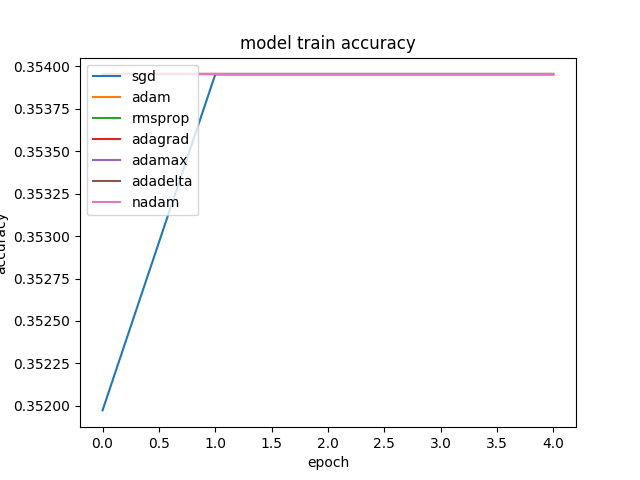
\includegraphics[width=\textwidth]{low_maxword_total_train_accuracy.png}
        \caption{Train accuracy}
        \label{fig:taomw}
    \end{subfigure}
     %add desired spacing between images, e. g. ~, \quad, \qquad, \hfill etc. 
      %(or a blank line to force the subfigure onto a new line)
    \begin{subfigure}[b]{0.7\textwidth}
        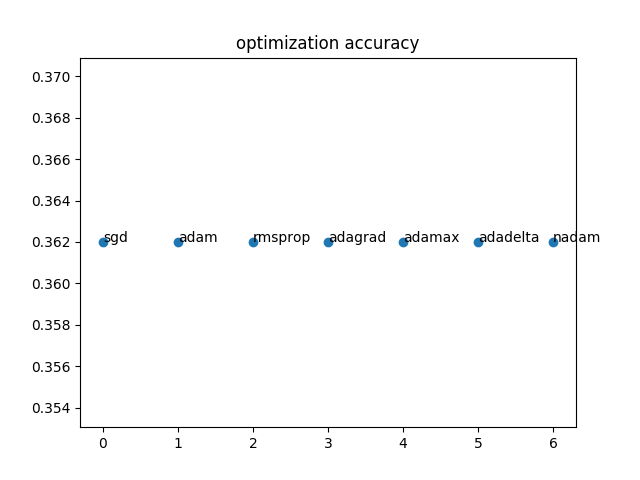
\includegraphics[width=\textwidth]{low_maxword_total_opt_acc.png}
        \caption{Test accuracy}
        \label{fig:teaomw}
    \end{subfigure}
    \caption{Results with low amount of words processed}\label{fig:ovlowwords}
\end{figure}

\begin{figure}[H]
    \centering
    \begin{subfigure}[b]{0.7\textwidth}
        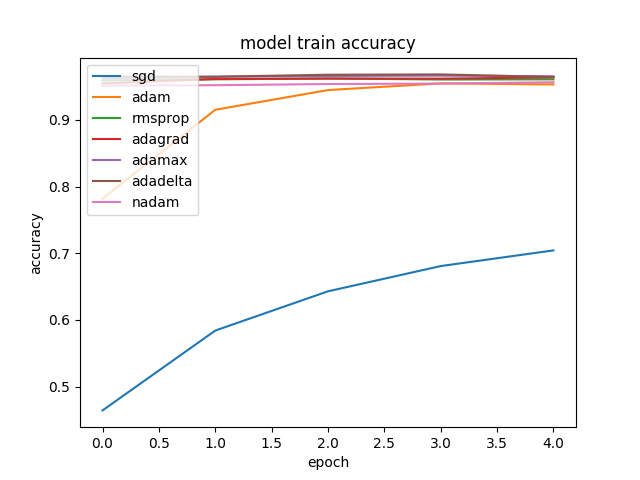
\includegraphics[width=\textwidth]{high_maxword_total_train_accuracy.png}
        \caption{Train accuracy}
        \label{fig:tahmw}
    \end{subfigure}
     %add desired spacing between images, e. g. ~, \quad, \qquad, \hfill etc. 
      %(or a blank line to force the subfigure onto a new line)
    \begin{subfigure}[b]{0.7\textwidth}
        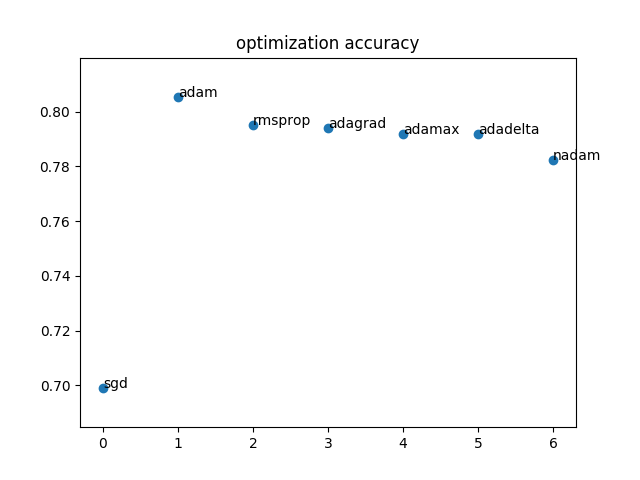
\includegraphics[width=\textwidth]{high_maxword_total_opt_acc.png}
        \caption{Test accuracy}
        \label{fig:teahmw}
    \end{subfigure}
    \caption{Results with high amount of words processed}\label{fig:rhmw}
\end{figure}

\begin{figure}[H]
    \centering
    \begin{subfigure}[b]{0.7\textwidth}
        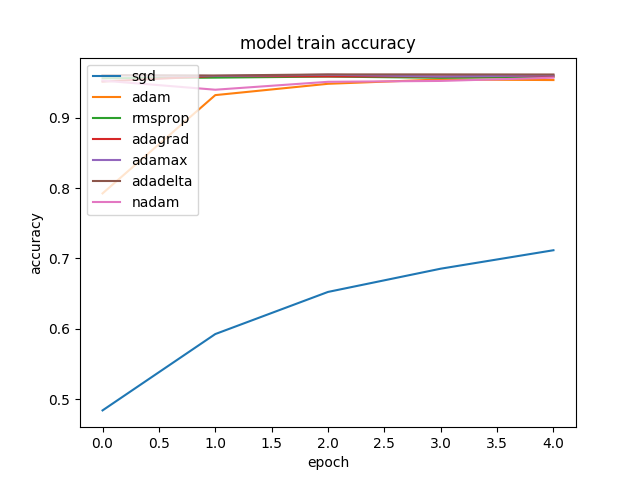
\includegraphics[width=\textwidth]{1layertotaltrainacc.png}
        \caption{Train accuracy}
        \label{fig:onelayertrainacc}
    \end{subfigure}
     %add desired spacing between images, e. g. ~, \quad, \qquad, \hfill etc. 
      %(or a blank line to force the subfigure onto a new line)
    \begin{subfigure}[b]{0.7\textwidth}
        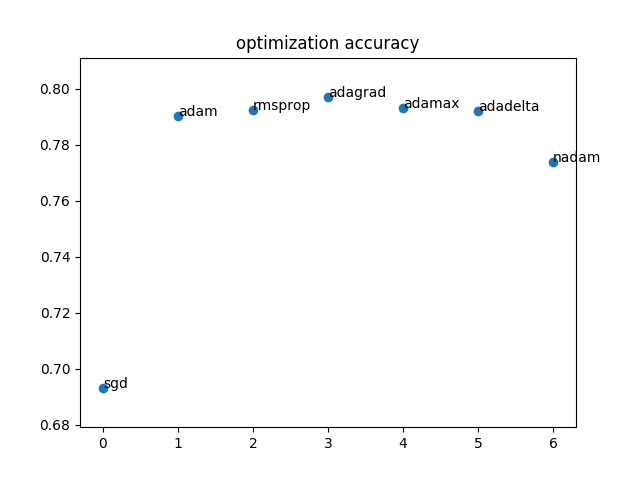
\includegraphics[width=\textwidth]{1layer_total_opt_acc.png}
        \caption{Test accuracy}
        \label{fig:onelayertestacc}
    \end{subfigure}
    \caption{Results with one hidden layer}\label{fig:rol}
\end{figure}

\begin{figure}[H]
    \centering
    \begin{subfigure}[b]{0.7\textwidth}
        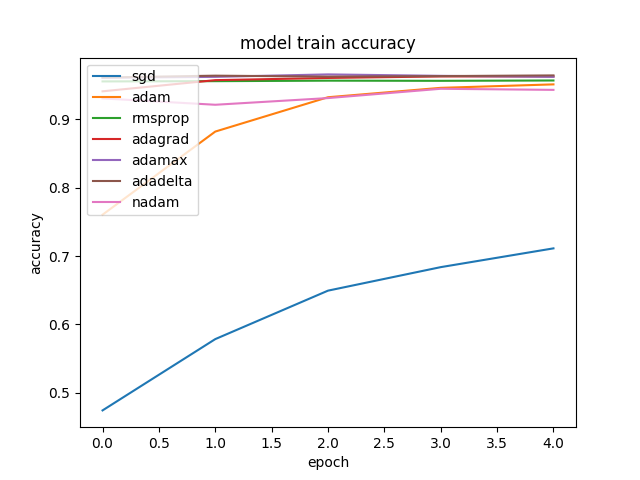
\includegraphics[width=\textwidth]{2layers20481024trainacc.png}
        \caption{Train accuracy}
        \label{fig:twolayertrainacc}
    \end{subfigure}
     %add desired spacing between images, e. g. ~, \quad, \qquad, \hfill etc. 
      %(or a blank line to force the subfigure onto a new line)
    \begin{subfigure}[b]{0.7\textwidth}
        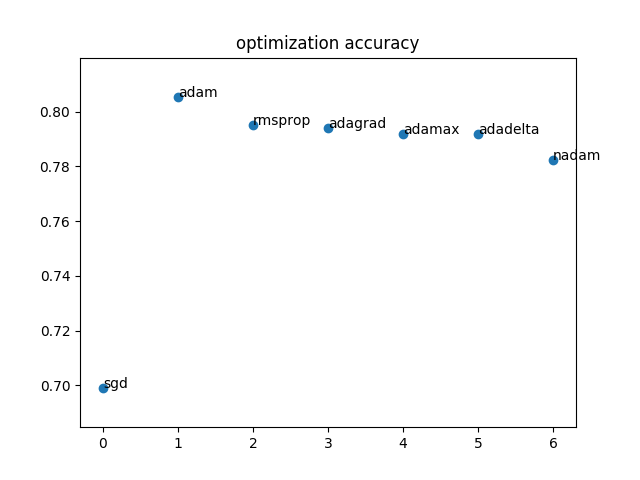
\includegraphics[width=\textwidth]{high_maxword_total_opt_acc.png}
        \caption{Test accuracy}
        \label{fig:twolayertestacc}
    \end{subfigure}
    \caption{Results with two hidden layers}\label{fig:rtl}
\end{figure}


\begin{figure}[H]
    \centering
    \begin{subfigure}[b]{0.7\textwidth}
        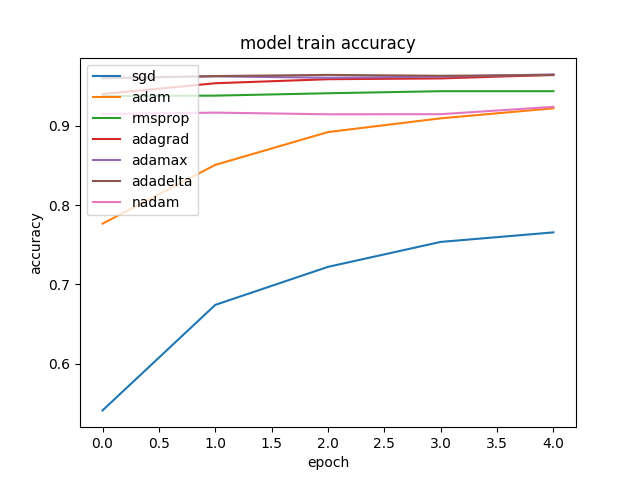
\includegraphics[width=\textwidth]{smallbatchtrainacc.png}
        \caption{Train accuracy}
        \label{fig:smalltrainacc}
    \end{subfigure}
     %add desired spacing between images, e. g. ~, \quad, \qquad, \hfill etc. 
      %(or a blank line to force the subfigure onto a new line)
    \begin{subfigure}[b]{0.7\textwidth}
        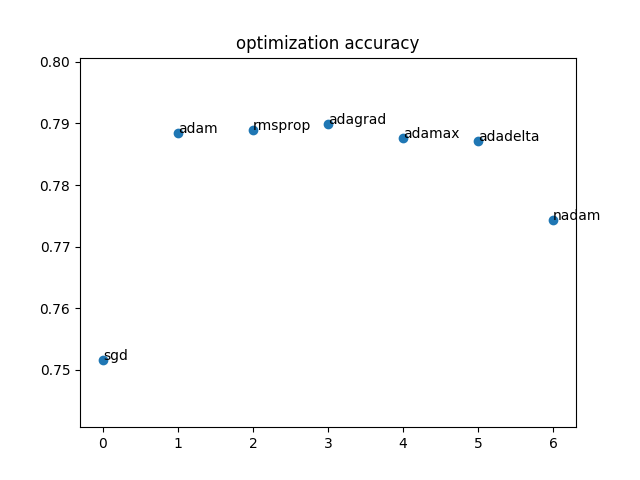
\includegraphics[width=\textwidth]{smalbatchtestacc.png}
        \caption{Test accuracy}
        \label{fig:smalltestacc}
    \end{subfigure}
    \caption{Results with small batch size of 8}\label{fig:rsb}
\end{figure}


\begin{figure}[H]
    \centering
    \begin{subfigure}[b]{0.7\textwidth}
        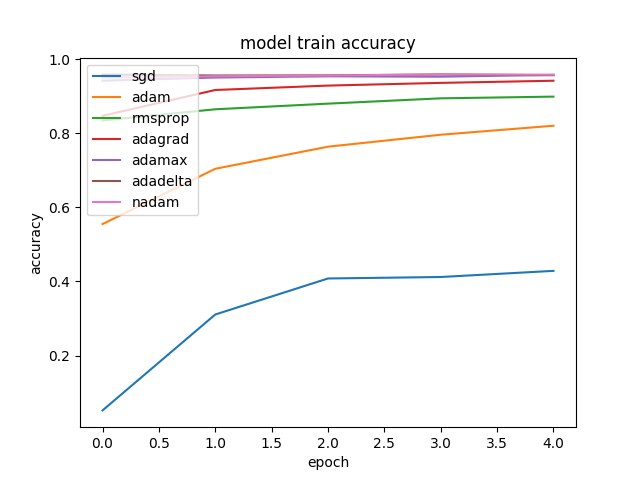
\includegraphics[width=\textwidth]{largebatchtraing.png}
        \caption{Train accuracy}
        \label{fig:largebathctrain}
    \end{subfigure}
     %add desired spacing between images, e. g. ~, \quad, \qquad, \hfill etc. 
      %(or a blank line to force the subfigure onto a new line)
    \begin{subfigure}[b]{0.7\textwidth}
        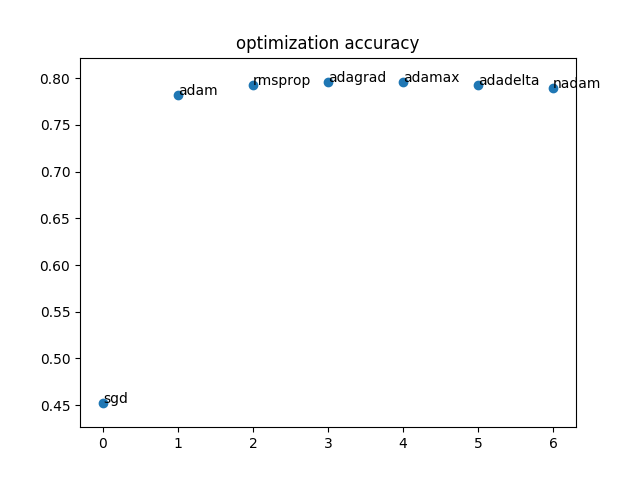
\includegraphics[width=\textwidth]{largebatchtestacc.png}
        \caption{Test accuracy}
        \label{fig:largetestacc}
    \end{subfigure}
    \caption{Results with large batch size of 512}\label{fig:rlb}
\end{figure}



\begin{figure}[H]
    \centering
    \begin{subfigure}[b]{0.7\textwidth}
        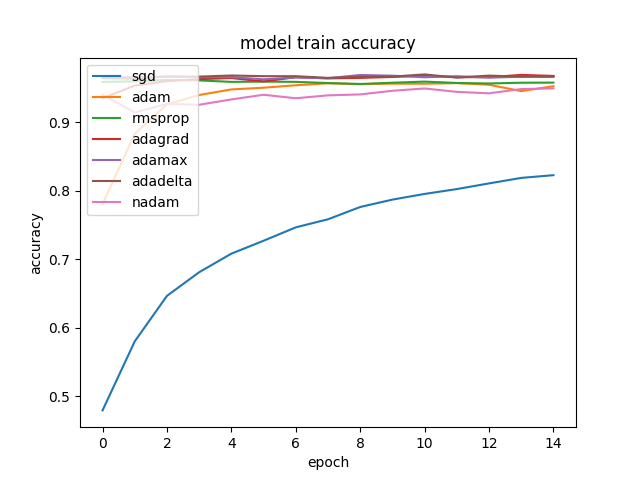
\includegraphics[width=\textwidth]{15epochstrainacc.png}
        \caption{Train accuracy}
        \label{fig:15epochtrain}
    \end{subfigure}
     %add desired spacing between images, e. g. ~, \quad, \qquad, \hfill etc. 
      %(or a blank line to force the subfigure onto a new line)
    \begin{subfigure}[b]{0.7\textwidth}
        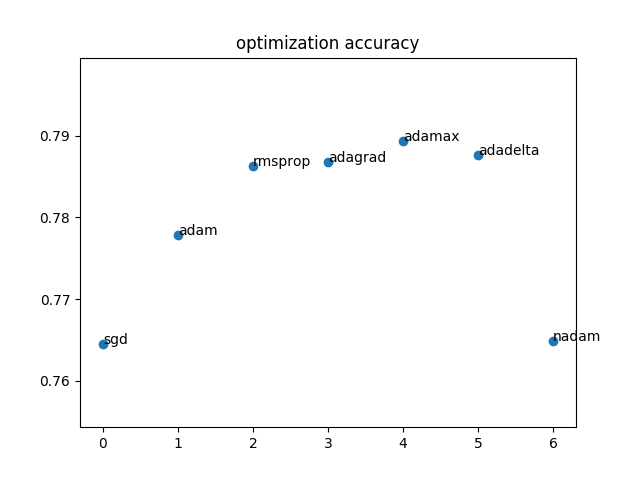
\includegraphics[width=\textwidth]{15epochstestacc.png}
        \caption{Test accuracy}
        \label{fig:15epochtest}
    \end{subfigure}
    \caption{Results using 15 epochs}\label{fig:r15e}
\end{figure}





\end{document}
